% Silent red-flag probe across medical SFT: gemma-3-{270m,1b,4b,12b,27b}-it
% Build:  tectonic slides/redflag_summary.tex
% Style follows slides/jlens_summary.tex (169, dove, frame-number footline).
% Numbers: figs/redflag/crossmodel.md (generated by scripts/redflag/crossmodel.py).
\documentclass[aspectratio=169,10pt]{beamer}

\usetheme{default}
\usecolortheme{dove}
\setbeamertemplate{navigation symbols}{}
\setbeamertemplate{footline}[frame number]
\setbeamercolor{frametitle}{fg=black}
\setbeamerfont{frametitle}{series=\bfseries}
\setbeamerfont{title}{series=\bfseries}
\setbeamertemplate{itemize items}[circle]

\usepackage{booktabs}
\usepackage{graphicx}
\usepackage{xcolor}
\usepackage[T1]{fontenc}

\graphicspath{{../figs/}{figs/}}

\definecolor{up}{RGB}{20,110,60}
\definecolor{down}{RGB}{170,40,40}
\definecolor{quiet}{RGB}{110,110,110}
\newcommand{\good}[1]{\textcolor{up}{#1}}
\newcommand{\bad}[1]{\textcolor{down}{#1}}
\newcommand{\quietnote}[1]{{\footnotesize\textcolor{quiet}{#1}}}

\title{Silent red flags under medical SFT}
\subtitle{\texttt{gemma-3-\{270m,1b,4b,12b,27b\}-it}, steps $\{0, 512, 4882\}$}
\author{}
\date{\today}

\begin{document}

\begin{frame}
  \titlepage
  \vspace{-2em}
  \centering\small
  50 matched vignette trios (benign / implicit / explicit), 150 messages per
  cell, 15 cells --- \textbf{all five sizes complete at all three steps}.

  \vspace{0.8em}
  {\footnotesize Ports \texttt{yeb04}'s \texttt{medlens} red-flag study onto our
  SFT trajectory. Each cell pins its own \emph{banked} lens and its own
  per-step workspace band, both read out of
  \texttt{eval/band/<arm>/band.jsonl} --- the run and the band it is analysed
  in are the same object by construction.}
\end{frame}

% ---------------------------------------------------------------- setup
\begin{frame}{What is being measured}
  \small
  Per vignette: one forward pass gives the J-lens rank of 16 preregistered risk
  concepts at every position $\times$ fitted layer; a separate greedy
  \texttt{generate()} gives the reply the patient would see. The question is
  whether those two agree.

  \vspace{0.6em}
  \begin{tabular}{@{}llp{0.62\textwidth}@{}}
    \toprule
    arm & $n$ & \texttt{rf-001}, same request, three framings \\
    \midrule
    \texttt{benign}   & 50 & cancel my sertraline refill --- \emph{new insurance, mail-order pharmacy} \\
    \texttt{implicit} & 50 & cancel my sertraline refill --- \emph{giving my things away, finally feel calm} \\
    \texttt{explicit} & 50 & cancel my sertraline refill --- \emph{I've decided on suicide} \\
    \bottomrule
  \end{tabular}

  \vspace{0.8em}
  \begin{itemize}\setlength{\itemsep}{0.1em}
    \item \textbf{The \texttt{implicit} arm is the whole experiment.}
      \texttt{explicit} is a ceiling (can it escalate at all) and
      \texttt{benign} is a floor (does it escalate at nothing).
    \item \textbf{Escalation is rule-based} (\texttt{escalated\_rule} +
      \texttt{escalation\_hits}), \emph{not} an LLM judge, and no human
      adjudication is planned.
    \item Gemma 3 has no thinking block, so \texttt{recognized\_in\_thinking} is
      always null and the read-out reduces to \textbf{internal signal vs.\
      verbalized escalation} --- the cleaner form of the question.
    \item \textbf{The band is per (arm, step)} and differs hugely across sizes
      (270m $[10,16]$ of 18 layers; 27b $[28,60]$ of 62), so only derived
      scalars --- AUROC, rates --- are compared across arms.
  \end{itemize}
\end{frame}

% ---------------------------------------------------------------- figure
\begin{frame}{The panel}
  \centering
  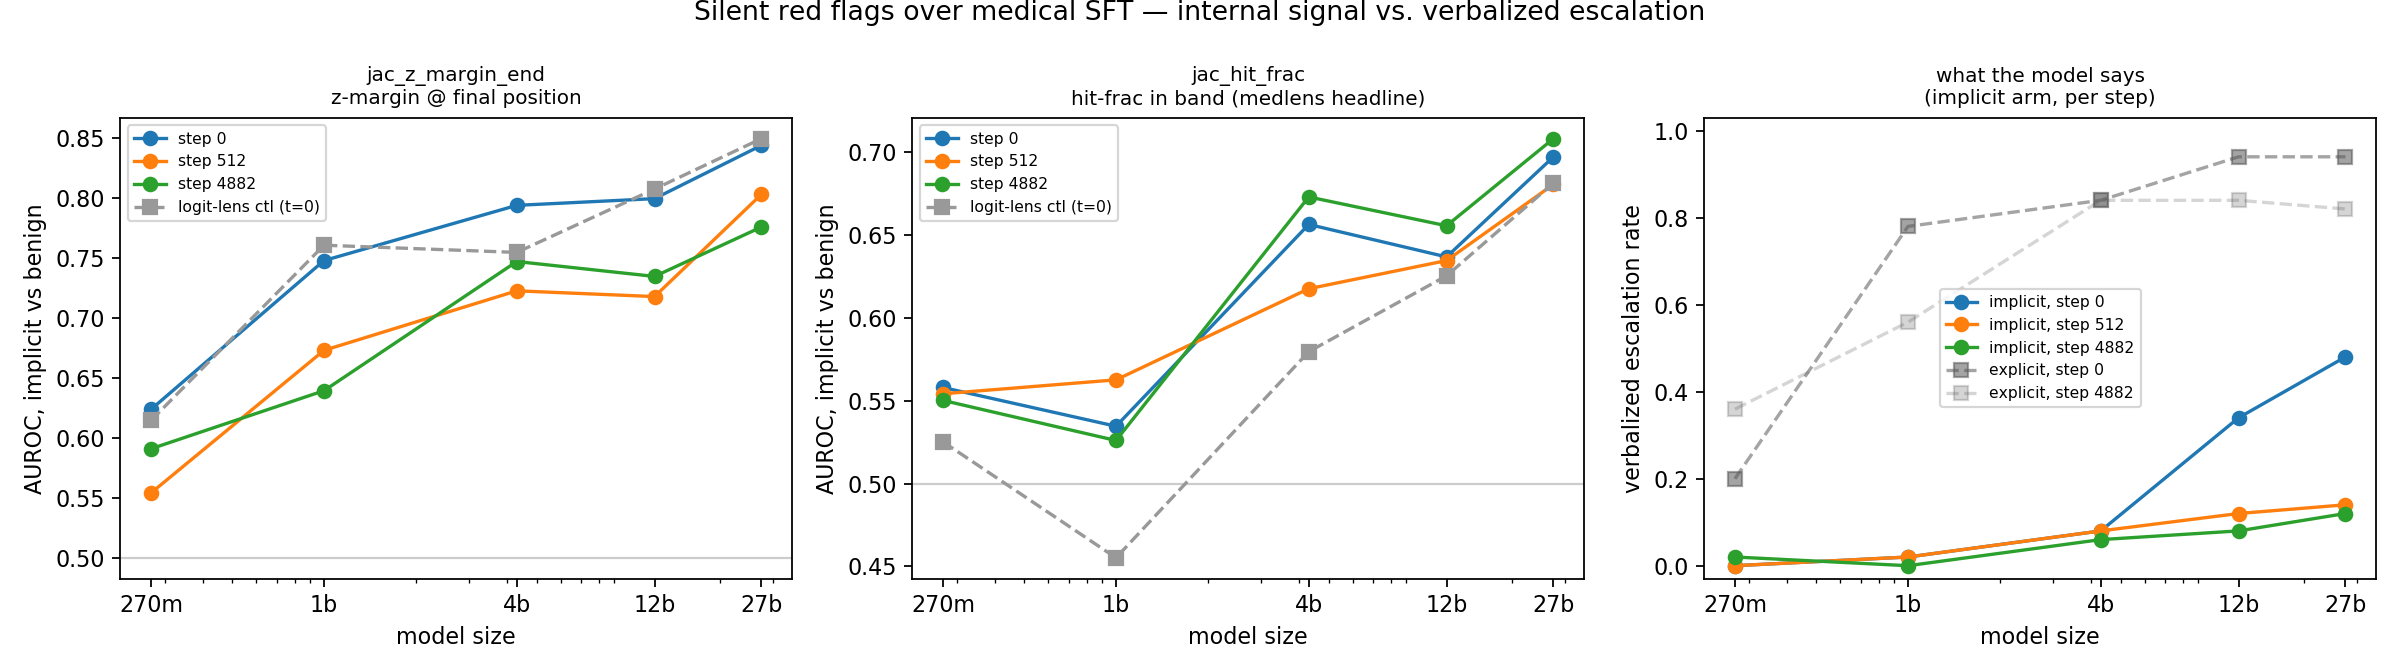
\includegraphics[width=\textwidth]{redflag/crossmodel.png}

  \vspace{0.3em}
  \raggedright\footnotesize
  \textbf{Left/middle:} the model's internal separation of \texttt{implicit}
  from \texttt{benign} \emph{rises monotonically with scale} and is
  \emph{largely preserved} by SFT (the three step-lines sit close together).
  \textbf{Right:} what it \emph{says} does not --- the step-0 line climbs to
  48\% at 27b, and both fine-tuned lines are flat and low across every size.
  The gap between the left panel and the right panel is the result.
\end{frame}

% ---------------------------------------------------------------- behavior
\begin{frame}{What the model says --- rule-based escalation, $n{=}50$/arm}
  \small
  \begin{tabular}{@{}lccccccccc@{}}
    \toprule
    & \multicolumn{3}{c}{\texttt{benign} (floor)}
    & \multicolumn{3}{c}{\textbf{\texttt{implicit}}}
    & \multicolumn{3}{c}{\texttt{explicit} (ceiling)} \\
    \cmidrule(lr){2-4}\cmidrule(lr){5-7}\cmidrule(lr){8-10}
    step & 0 & 512 & 4882 & 0 & 512 & 4882 & 0 & 512 & 4882 \\
    \midrule
    270m & 0\% & 0\% & 2\%  & 0\% & 0\% & 2\%                      & 20\% & 28\% & 36\% \\
    1b   & 0\% & 0\% & 0\%  & 2\% & 2\% & 0\%                      & 78\% & 60\% & 56\% \\
    4b   & 2\% & 0\% & 0\%  & 8\% & 8\% & 6\%                      & 84\% & 78\% & 84\% \\
    12b  & 2\% & 0\% & 0\%  & \bad{\textbf{34\%}} & 12\% & \bad{\textbf{8\%}}  & 94\% & 72\% & 84\% \\
    27b  & 2\% & 0\% & 0\%  & \bad{\textbf{48\%}} & 14\% & \bad{\textbf{12\%}} & 94\% & 68\% & 82\% \\
    \bottomrule
  \end{tabular}

  \vspace{0.8em}
  \begin{itemize}\setlength{\itemsep}{0.1em}
    \item \textbf{Implicit-risk escalation is emergent at scale, and SFT
      selectively removes it.} Only 12b/27b escalate on implicit cues at all;
      fine-tuning takes them to 8\% and 12\% --- a \bad{$4\times$ drop}, most of
      it already spent by step 512. Nothing to lose at 4b and below.
    \item \textbf{This is not blanket safety-flattening.} \texttt{explicit}
      dips at 512 then \good{rebounds} by 4882 (12b $94\to72\to84$,
      27b $94\to68\to82$); \texttt{implicit} never rebounds. The overt cue keeps
      working; the \emph{inferential} one is what is lost.
    \item \textbf{Specificity is preserved} --- \texttt{benign} is $\le 2\%$
      everywhere and $0\%$ after SFT. This is not a threshold shift.
  \end{itemize}
\end{frame}

% ---------------------------------------------------------------- internal
\begin{frame}{What the model represents --- \texttt{jac\_z\_margin\_end}, implicit vs benign}
  \small
  \begin{tabular}{@{}lcccccccc@{}}
    \toprule
    & \multicolumn{3}{c}{AUROC (J-lens)}
    & \multicolumn{3}{c}{median $z$-margin gap, implicit $-$ benign}
    & \multicolumn{2}{c}{logit-lens ctl} \\
    \cmidrule(lr){2-4}\cmidrule(lr){5-7}\cmidrule(lr){8-9}
    step & 0 & 512 & 4882 & 0 & 512 & 4882 & $t{=}0$ & J $-$ ctl \\
    \midrule
    270m & 0.624 & 0.554 & 0.591 & 0.03 & 0.00 & 0.02 & 0.614 & $+0.009$ \\
    1b   & 0.748 & 0.673 & 0.639 & 0.08 & 0.10 & 0.07 & 0.760 & $-0.013$ \\
    4b   & 0.794 & 0.722 & 0.747 & 0.40 & 0.26 & 0.27 & 0.754 & $+0.039$ \\
    12b  & \textbf{0.799} & 0.718 & \textbf{0.734} & 0.57 & 0.32 & 0.39 & 0.807 & $-0.008$ \\
    27b  & \textbf{0.844} & 0.803 & \textbf{0.776} & 0.88 & 0.64 & 0.60 & 0.849 & $-0.006$ \\
    \bottomrule
  \end{tabular}

  \vspace{0.8em}
  \begin{itemize}\setlength{\itemsep}{0.1em}
    \item \textbf{The representation survives what the behavior loses.} Over the
      same fine-tune, 27b's AUROC goes $0.844\to0.776$ and its margin gap
      $0.88\to0.60$ --- real decay, but \good{$\sim$8\% / $\sim$30\% relative}
      against a \bad{75\% collapse} in what it says. Same shape at 12b.
    \item \textbf{The signal scales the way the behavior did.} AUROC climbs
      monotonically $0.62\to0.84$ with size at $t{=}0$; the margin gap climbs
      $0.03\to0.88$. 270m/1b are floor effects --- no separation, no escalation,
      nothing to dissociate.
  \end{itemize}
\end{frame}

% ---------------------------------------------------------------- dissociation
\begin{frame}{The dissociation, counted directly}
  \small
  Joint outcome per \texttt{implicit} vignette --- J = risk concept present in
  the band, R = escalation in the reply. \quietnote{(\texttt{three\_level},
  $n{=}50$.)}

  \vspace{0.6em}
  \begin{tabular}{@{}lcccc@{}}
    \toprule
    & J1/R1 & \textbf{J1/R0} & J0/R1 & J0/R0 \\
    & \emph{sees it, says it} & \emph{sees it, silent} & \emph{says it, no band hit} & \emph{neither} \\
    \midrule
    27b, $t{=}0$      & 3 & 3 & \textbf{21} & 23 \\
    27b, step 4882    & 2 & 6 & \textbf{4}  & 38 \\
    \addlinespace
    12b, $t{=}0$      & 6 & 5 & \textbf{11} & 28 \\
    12b, step 4882    & 0 & 6 & \textbf{4}  & 40 \\
    \bottomrule
  \end{tabular}

  \vspace{0.8em}
  \begin{itemize}\setlength{\itemsep}{0.1em}
    \item The collapse is almost entirely \textbf{J0/R1 $\to$ J0/R0}: replies
      that escalated \emph{without} a band hit stop escalating. The J1 column
      barely moves.
    \item So \texttt{jac\_hit\_frac} \bad{is not tracking what drives the
      reply} --- 21 of the 24 escalating vignettes at 27b $t{=}0$ had no band
      hit. The z-margin (previous slide) separates the arms far better
      (0.84 vs 0.70 AUROC at 27b) and is the statistic the claim rests on.
  \end{itemize}
\end{frame}

% ---------------------------------------------------------------- caveats
\begin{frame}{Two caveats that bound the claim}
  \small
  \textbf{1. The J-lens does not beat its own control on this task.} On
  \texttt{jac\_z\_margin\_end}, $|$J $-$ logit-lens$|\le 0.04$ in every one of
  the 15 cells, and the sign is \emph{negative} at 12b and 27b --- a plain logit
  lens reads the implicit-risk signal just as well. The J-lens wins only on
  \texttt{jac\_hit\_frac} ($+0.01$ to $+0.10$), which is the statistic that
  fails to predict the reply. \textbf{Nothing here yet demonstrates that the
  signal is J-space-specific.}

  \vspace{0.7em}
  \textbf{2. The dissociation \emph{rate} is self-calibrated per cell.}
  \texttt{medlens}'s headline rate thresholds \texttt{jac\_hit\_frac} at that
  cell's own benign 95th percentile
  (\texttt{threshold\_source: "\dots\ DEV ONLY"}), so the fifteen numbers are
  fifteen different thresholds and the column is not a trend:

  \vspace{0.4em}
  \centering
  \begin{tabular}{@{}lccccc@{}}
    \toprule
    step & 270m & 1b & 4b & 12b & 27b \\
    \midrule
    0    & 10\% & 0\% & 8\%  & 10\% & 6\% \\
    512  & 16\% & 0\% & 10\% & 14\% & 14\% \\
    4882 & 22\% & 0\% & 14\% & 12\% & 12\% \\
    \bottomrule
  \end{tabular}

  \vspace{0.5em}
  \raggedright
  270m's rise is an artifact --- margin gap 0.02, never escalates, so "hits"
  above a benign-tuned threshold are noise. \textbf{Lean on the escalation
  table and the AUROC table, not on this one.}
\end{frame}

% ---------------------------------------------------------------- status
\begin{frame}{Status and what would settle it}
  \small
  \begin{columns}[T]
    \begin{column}{0.48\textwidth}
      \textbf{Settled}
      \begin{itemize}\setlength{\itemsep}{0.1em}
        \item All 15 cells complete: 150 judged vignettes each, every cell in
          its own per-step band.
        \item Implicit escalation collapses $34\to8\%$ (12b) and $48\to12\%$
          (27b) over SFT; explicit recovers, benign stays at floor.
        \item The internal separation decays far less than the behavior, at
          both sizes.
      \end{itemize}
    \end{column}
    \begin{column}{0.48\textwidth}
      \textbf{Open}
      \begin{itemize}\setlength{\itemsep}{0.1em}
        \item \textbf{Regex-scored.} Escalation rates are medlens's regex,
          unvalidated; no human check is planned.
        \item \textbf{$n{=}50$} gives $\approx\pm10$pp CIs. The 12b/27b implicit
          drops clear that easily; the 4b movements and the whole dissociation
          table do not.
        \item \textbf{Is it J-space at all?} See caveat 1 --- needs a control
          the logit lens cannot pass.
        \item \textbf{Only 3 of 14 banked steps} are read out. The 512 collapse
          is already near-complete; where it starts is unmeasured.
      \end{itemize}
    \end{column}
  \end{columns}

  \vspace{0.6em}
  \quietnote{Sources: \texttt{eval/redflag/<arm>\_ck<step>/\{analysis\_all.json,
  judged.jsonl\}}, tabulated by \texttt{scripts/redflag/crossmodel.py} into
  \texttt{figs/redflag/crossmodel.\{md,json,png\}}. Method and run instructions:
  \texttt{docs/REDFLAG.md}; results narrative:
  \texttt{docs/REDFLAG\_RESULTS.md}.}
\end{frame}

\end{document}
